% Improving Locality of Unstructured Mesh Algorithms on GPUs

\noindent Unstructured mesh solvers, particularly applied to the solution of 
finite difference, finite volume or finite element algorithms, form the basis 
of numerical simulation applications in a vast area of important scientific 
domains, from modeling the flow of blood in the body, the flow past an aircraft, 
to ocean circulation and the simulation of Tsunamis. Significant computational 
resources are required for the execution of numerical algorithms on these highly 
detailed (usually three-dimensional) meshes. The solution involves repeatedly 
iterating over millions of elements (such as mesh edges, nodes, etc.) to reach 
the desired accuracy or resolution. The key distinguishing feature of these 
applications is that operations over mesh elements make use of explicit 
connectivity information between elements to access data defined on neighboring 
elements. This is in contrast to the use of stencils in structured-mesh 
applications where the regular geometry of the mesh implicitly provides the 
connectivity information. As such, iterations over unstructured-meshes lead to 
highly irregular patterns of data accesses over the mesh, characterized by 
indirect array accesses. For example, computations over the mesh involve 
iterating over elements of a set (e.g. faces), performing the same computations, 
on different data, accessing/modifying data on the set which they operate on 
(e.g. fluxes defined on the faces), or, using indirections accessing/modifying 
data defined on other sets (such as coordinate data on connected vertices). 
These indirect accesses are particularly difficult to parallelize when multiple 
threads may try to modify the same data, leading to data races. 

Previous work has utilized one of three approaches for handling data races 
during parallelization~\cite{LULESH:spec,miniaero}: (1) use coloring where the 
iteration set is ``colored'' such that no two iterations of the same color 
modify the same mesh element indirectly, followed by parallel execution of the 
iterations with the same color, (2) use large temporary datasets to stage 
increments without race conditions, and a separate step to gather the 
increments, or (3) use atomics to handle race conditions. However, the amount 
of parallelism, and especially the data locality available to be exploited with 
the above methods have become increasingly limited on modern and emerging 
massively parallel multi-core and many-core architectures. The performance gains 
have been limited particularly on many-core processors such as GPUs with 
thousands of low-power cores, but with modest memory-bandwidth. Thus, reducing 
data movement and exploiting memory locality during execution is vital on such 
devices. On GPUs, the first two techniques, coloring or using temporary 
datasets, end up with poor data locality as one cannot have good data reuse in 
both reading data as well as writing data without conflicts. The third method, 
atomics, are much more expensive operations than regular memory transactions and 
therefore usually lead to low throughput. 

In this paper we explore novel data-movement avoiding and locality exploiting 
algorithms for improving performance of unstructured-mesh applications on GPUs. 
Identifying that the throughput of memory transactions is the main bottleneck, 
we demonstrate how superior execution strategies can be obtained by utilizing 
a combination of techniques from (1) element reordering at thread-block level, 
(2) use of GPU shared memory as an explicitly managed cache and (3) use of 
partitioning algorithms for thread-block formation. We show how these allow us 
to maximize data re-use to the higher-bandwidth shared memory, and optimize 
access patterns to both shared and GPU global memory. More specifically, we make 
the following contributions:
\begin{enumerate}
\item We adopt a caching mechanism on the GPU that loads indirectly accessed 
elements into GPU shared memory. Then use a two-level ``hierarchical coloring'' 
approach to avoid data races, but improve locality over traditional global 
coloring. 

\item We design a reordering algorithm based on graph partitioning that 
increases data reuse within a thread block, also further increasing shared 
memory utilization. 

\item Finally, we apply the above techniques and optimizations to a number of 
representative unstructured-mesh applications to investigate performance on 
modern GPUs, contrasting performance improvements over the state-of-the-art. 
\end{enumerate}

\noindent We demonstrate how the above locality-exploiting algorithms provide 
performance improvements of up to 75\% compared to the state-of-the-art on the 
latest NVIDIA Pascal and Volta GPUs. The algorithms are implemented as an 
open-source software library~\cite{opt-library} which can be used for improving 
performance of existing or new unstructured-mesh applications. 

The rest of the paper is organized as follows: the remainder of Section
\ref{introduction} introduces the basic concepts of unstructured meshes, 
numerical methods based on them and a discussion on related works, Section 
\ref{parallelisation-on-gpu} describes our optimized algorithms and the 
motivation leading to the design. Section \ref{performance} presents the 
performance analysis of the algorithms with experimental results. Finally, in 
Section \ref{conclusion}, we present conclusions from this research. 
%\ref{library-implementation} contains a brief description of the structure of 
%the open source library.


\subsection{Background}\label{sec:background}
\subsubsection{Unstructured meshes}\label{unstructured-meshes}

\noindent Unstructured meshes can be abstractly viewed as a collection of sets 
(e.g. nodes, edges, cells, etc.), data defined on these sets (e.g. fluxes, 
coordinates, velocities), and explicit connectivity information between 
sets. The connectivity information, declared as mapping tables are required for 
determining the neighbors of a set element. If we represent sets as consecutive 
indices from zero to the size of the set, then the mapping between two 
sets is represented as an array which stores the index of set elements in the 
second set of the mapping (referred to as the to-set) for every set element of 
the first set (known as the from-set). For the majority of such applications, the number of to-set elements connected to each from-set element is fixed (e.g. all edges have two vertices). For example consider the mesh illustrated 
in Figure~\ref{fig:unstructured}. Figure~\ref{fig:mapping} details how part of 
the mappings from edges to cells are defined for this mesh. Given such a 
mapping, we can access the index of those elements which are connected to the 
current element of the from-set from other sets (the to-sets of the mappings). 

The computations on the mesh are declared as a loop over the elements of a set, 
executing some block of computation on each set element (i.e. an elemental kernel), 
while accessing data directly on the iteration set or indirectly through a 
mapping.  If a loop over a set only write to data defined on that set during the 
elemental kernel, then each iteration of the loop could run in parallel. 
However, for kernels which indirectly increment data, there may be multiple 
from-set iterations that update the same to-set element. Such indirect-loops are 
common in finite volume and finite element applications over 
unstructured-meshes: e.g. when updating state variables in cells using fluxes 
across faces, or when doing matrix assembly. The parallelization of indirect 
loops are non-trivial as the exact elements leading to data races cannot be 
determined from compile time-information, given they are driven by the 
structure of the mesh in general and the mapping tables in particular, which are 
read in during run-time. 

% The sole focus of the research is this paper is this indirect-loop data access 
% pattern. 


\begin{figure}
\centering

\includegraphics[width=4cm]{fig/svg/unstructured.eps}
\caption{Unstructured mesh, the arrow represents the mapping tells $e_i$ is
  connected to $c_j$ and $c_k$.}
\label{fig:unstructured}
\end{figure}



\begin{figure}
\centering
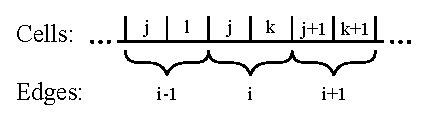
\includegraphics[width=6cm]{fig/svg/mapping.eps}
\caption{A part of the mapping from edges to cells.}
\label{fig:mapping}
\end{figure}


Some restrictions that apply is also worth noting here. The first is the use of 
only a single level of mappings. This means that every piece of data that is 
accessed during an iteration over a set is either defined directly on that set, 
or is accessed through at most one level of indirection. However, this 
restriction does not exclude applications using nested indirections, since a 
mapping table can be created to contain the indexes that we access through 
multiple mappings. The second restriction is that the result of the operations 
on the sets are independent from the order of processing the elements of the 
sets (within machine precision). This restriction enables to exploit the 
maximum opportunities for parallelization given that the accuracy of the 
algorithms do not depend on the order of execution. Finally, only  mappings with 
a fixed number of connections (or arity) are considered; such as edges to 
vertices (where the degree is always 2), unlike for a vertices to vertices 
mapping, where this will vary. The natural formalization of most FEM and FV 
algorithm uses mappings with fixed number of connections.


\subsection{Related Work}\label{sec:related-works}
\noindent
Algorithms defined on unstructured meshes form an important 
class of applications at many organizations. It is one of the seven dwarfs -- 
common computation-communication patterns or motifs occurring in parallel 
numerical applications -- identified by Colella in 2004~\cite{Colella2004}. 
Discretizations such as finite volumes (FV) or finite elements (FE) often rely 
on these meshes to deliver high-quality results. Indeed there is a large number 
of papers detailing such algorithms, and a wide range of commercial, government, 
and academic research codes (e.g. OpenFOAM~\cite{OpenFoamUserGuide}, Rolls-Royce 
Hydra~\cite{moinier2002edge}, FUN3D~\cite{biedron2017fun3d}). All such 
applications use unstructured meshes in some shape or form, and are often used 
for large experiments, consisting of millions or even billions of mesh elements. 
These codes are generally critical to production and consume large portions of 
high-performance computing systems time. As such, the efficient execution of 
these applications on the parallel architectures of the day has been and 
continues to be crucial to the organizations and stake-holders that have 
invested in them for continued scientific delivery. Over the years, many works 
have discussed and presented techniques for efficient implementations, initially 
focusing on traditional CPU architectures~\cite{mavriplis2002parallel, 
jin1999openmp}, then many-core processors such as GPUs (as we discuss below), 
and even architectures such as FPGAs~\cite{nagy2014accelerating, 
akamine2012reconfigurable}. Many libraries have also been developed targeting 
unstructured-mesh solvers, from classical libraries~\cite{trilinos, PETSc} to 
domain specific languages~\cite{devito2011liszt, giles2012op2, pyfr2016}. 

The adoption of GPUs for these kind of computations has already led to 
considerable speedups over traditional CPU architectures due to the 
massive parallelism available on GPUs~\cite{Reguly2015, ELSEN200810148, 
cohen2009fast}. Other notable works have further looked at improving 
performance. Remacle et al. \cite{remacle2016gpu}, explores efficiently solving 
elliptic problems on unstructured hexahedral meshes on GPUs. They use shared 
memory for improving data locality, but advanced techniques, such as reordering 
and partitioning are not utilized. Work done by Castro et al. 
\cite{shallow_water} on implementing path-conservative Roe type high-order 
finite volume schemes to simulate shallow flows uses auxiliary accumulators to 
avoid data races while indirectly incrementing. Wu et al. 
\cite{wu2013complexity} introduce caching using the shared memory with 
partitioning (clustering), but do not use coloring. Instead they use a 
duplication method similar to that of LULESH and miniAero, as described below. 
Fu et al. \cite{fu2014architecting} also create contiguous patches (blocks) in 
the mesh to be loaded into shared memory, although they partition the nodes (the 
to-set) but not the elements (the from-set of the mapping). Furthermore, they do 
not load all data into shared memory, only what is inside the patch. Writing the 
result back to shared memory is done by a binary search for the column index and 
atomic adds, which leads to inefficiencies on the GPU. 

Parallel to the above work, the US Department of Energy labs have released a 
set of proxy applications that represent large internal production codes,
showing some of the computational and algorithmic challenges to be overcome on 
novel and emerging architectures Lulesh \cite{LULESH2:changes}, 
miniAero~\cite{miniaero}, BookLeaf~\cite{bookleaf}, MiniFE~\cite{minife}, 
PENNANT~\cite{pennant}. Out of this suite of codes there are three key 
approaches to handling data races: (1) allocate large temporary arrays where 
the intermediate results (i.e. the increments) are placed, avoiding any race 
conditions, followed by the use of a separate kernel to gather the results, 
(2) use atomics, (3) use coloring. These all lead to increased warp divergence 
and high data access latencies on GPUs; and the use of the temporary array also 
leads to more data allocations and movement, further constraining bandwidth. 

The research detailed in the present work is based on previous work 
in~\cite{op2}, where the OP2 library's GPU parallelization use shared memory on 
GPUs using CUDA for caching with a two level ``hierarchical'' coloring. However, 
we demonstrate superior execution strategies on GPUs with reordering of threads 
and data, to increase data reuse and maximize data locality. Instead of directly 
porting a specific application to use these techniques we present our methods 
as a classical library that can be used in general to accelerate unstructured 
mesh applications, and in particular the indirect increment algorithmic 
pattern, on GPUs. \textbf{[Is the utilization of this classical library 
presented in the paper given that we removed the appendix ? - Gihan]}

Most applications of interest for our work implements finite volume algorithms, 
and low order finite element algorithms, which has a lower computational 
intensity compared to the number of memory transactions. Thus our optimizations 
are targeted to avoid data movement, exploiting locality. In contrast high 
order finite element methods usually have significantly higher computational 
intensity, where there is a higher number of computations per data element 
accessed that can hide the cost of the memory access. While our techniques could 
potentially improve locality, memory bandwidth is less of a concern for such 
applications.


% In most finite volume algorithms, and low order finite element algorithms the 
% ratio of computations to number of bytes is relatively low - at least 
% compared to the ideal balance on modern GPUs. Therefore the proper usage of 
% the memory system for such simulations is crucial to get good performance. 
% High order finite elements usually have much higher computational 
% requirements, thus memory bandwidth is less of a concern. The throughput of 
% memory accesses is the main bottleneck for a large class of applications, thus 
% our goal is to lower the impact of the memory transactions. Since in most 
% applications of interest, there isn't enough computations to hide the cost of 
% memory movement, we can either increase the number of memory transactions in 
% flight (to more efficiently utilise bandwidth), or decrease the number of 
% memory transactions. To achieve the latter goal, a common technique is the use 
% of shared memory within CUDA thread blocks as an explicitly managed cache, 
% because it has much higher bandwidth and lower latency than global memory. The 
% challenge then is to maximise data re-use within shared memory, and optimise 
% access patterns to both shared and global memory.


